\subsection{The Additive Gaussian Noise Model}
By assuming the measurements are corrupted by the additive Gaussian noise, the linear estimation model can be written as 
\begin{equation}
\mathbf{d} \sim \text{Gaussian}( \mathbf{A} \mathbf{h}_t),
\end{equation}
\vspace{0.3cm}
where\\
\begin{tabular}{l c l}
$\mathbf{d}$ &=& a vector of measurements,\\
$\mathbf{A}$ &=& a linear forward operator,\\
$\mathbf{h}_t$ &=& the true bathymetry (depth). 
\end{tabular}

\vspace{0.3cm}
\noindent Therefore, the Gaussian noise $\boldsymbol{\epsilon}$ corrupted measurements $\mathbf{d}$ with variance $\nu$ is given by 
$$
\mathbf{d} = \mathbf{A} \mathbf{h}_t + \boldsymbol{\epsilon}.
$$



\subsection{Bathymetric Inversion Method}

As a beginning to approximate the topographic heights of the sea-floor,  we consider the following least-squares minimization problem,
\begin{equation}\label{LS}
\mathbf{\hat{h}}= \underset{\mathbf{h} \in \mathbb{R}^n}{\arg \min} \|  \mathbf{A}\mathbf{h} -  \mathbf{d} \|_2^2,
\end{equation}
where we minimize the data misfit between the forward prediction and the measurements in least-squares sense. 
This least-squares minimization problem \eqref{LS} can be solved using the following  MATLAB functions:
\begin{itemize}
\item[(1)]  Nonnegative least-squares method:  \verb|lsqnonneg(A,b)|  \\
\begin{center}
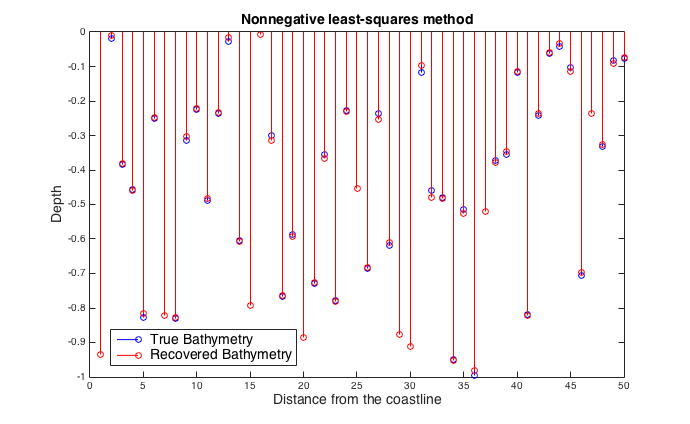
\includegraphics[scale=0.55]{img/NonLS.png} 
\end{center}
\item[(2)]  
\begin{center}
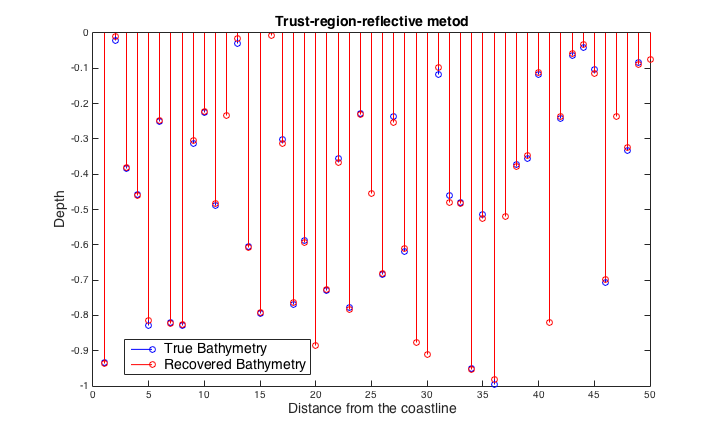
\includegraphics[scale=0.55]{img/trust_region.png} 
\end{center}

\end{itemize}
Challenges: What is the dimension of the $\mathbf{A}$? Is this a underdetermined or overdetermined system? If so, we have to consider the Tikhonov regularization,
$$
\hat{\Psi} = {\arg \min} \|  \mathbf{A}\mathbf{\Psi} -  \mathbf{d} \|_2^2  +  \alpha \| \mathbf{\Psi}\|_2^2,
$$
where $\alpha$ is a regularization parameter $(>0)$. 

\begin{center}
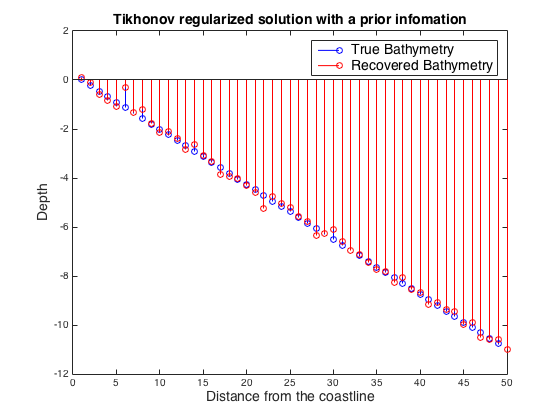
\includegraphics[scale=0.6]{img/Tikhnove_reg.png} 
\end{center}

Reference: I found a MATLAB package for analysis and solution of discrete ill-posed problems, which is available in http://www2.imm.dtu.dk/~pcha/Regutools/\\

\subsection{Help}

LSQR method: $\hat{\Psi}$ = lsqr(A,d,tol,maxit) it attempts to solve the least squares solution x that minimizes norm$(\mathbf{d}-\mathbf{A\Psi})$ Note that $\mathbf{A}$ need not be square.


Conjugate gradients: $\hat{\Psi}$ = cgs(A,b) attempts to solve the system of linear equations $\mathbf{A}\mathbf{\Psi} -  \mathbf{d}$ for $\Psi$.

